\documentclass[11pt]{article}

\setlength{\oddsidemargin}{0.0in}
\setlength{\evensidemargin}{0.0in}
\setlength{\topmargin}{0.0in}
\setlength{\headheight}{0.0in}
\setlength{\headsep}{0.0in}
\setlength{\topskip}{0.0in}
\setlength{\footskip}{0.5in}
\setlength{\textwidth}{6.5in}
\setlength{\textheight}{8.5in}
\setlength{\parskip}{1em}

\usepackage{wrapfig}
\usepackage{graphicx}
\usepackage{amsmath}
\usepackage{amssymb}
\graphicspath{ {./} }

\title{PCA Applied to Computer Vision \& Image Processing}
\author{Courtney Duquette \& Maya Shende}
\date{Due: May 9th, 2018}

\begin{document}

\maketitle

\section{Introduction} \label{introduction}
Principal Component Analysis (PCA) is a linear algebra tool used to see patterns in data that may be hard to otherwise see due to the data being high-dimensional or noisy. It can be used to extract groupings in data where the data represents non-numeric information, such as word counts. For example, PCA is used to find correlations between words in text, thus leading to correlations and similarities between larger texts. Another field in which PCA can be used is computer vision and image processing, the focus of this paper. Section \ref{background} will review some popular and prevalent uses of PCA in research and section \ref{pca-vision} will delve into the methodology behind how PCA can be used in interesting way in the field of computer vision. 

\section{Background} \label{background}
Lets start with a basic example of PCA and go through the different steps needed to analyze a set of data. PCA is used for finding patterns in a set of data that can either not be visualized or there is no discernible pattern. Let's look at the data matrix if we try to classify eight webpages into four categories based on key words. 

$$
\textbf{X} = 
\begin{bmatrix} 
10 &  4 & 14 &  8 & 17 & 12 &  5 & 18 \\
		13 &  1 & 12 & 10 &  3 &  5 &  0 & 14 \\	
  	        18 & 12 & 15 &  3 & 10 &  6 & 12 &  0 \\	
		 3 &  0 & 19 & 10 &  2 &  1 & 17 &  2 \\
\end{bmatrix}
$$
	
Based on looking at that matrix, there is no discernible pattern in the data so the PCA could be of some use. To perform PCA, start by finding the mean of the matrix. This is used to center the data about $(0,0)$. Below is the centered data.
 
$$
\textbf{X}_{C} = 
\begin{bmatrix} -1 & -7 &  3 & -3 &  6 &  1 & -6 &  7 \\
		5.75 & -6.25 & 4.75 & 2.75 & -4.25 & -2.25 & -7.25 & 6.75 \\	
  	        8.5 & 2.5 & 5.5 & -6.5 & 0.5 & -3.5 & 2.5 & -9.5 \\	
		-3.75 & -6.75 & 12.25 & 3.25 & -4.75 & -5.75 & 10.25 & -4.75 \\
\end{bmatrix}
$$

You can verify that the matrix is properly centered by taking the mean of the $\textbf{X}_{C}$ and ensuring it is the zero vector. It is important to normalize and center the data so you get the same range of values to use in the analysis. This can also help stabilize the convergence of the bias and weight. Once you have the centered data, you need to calculate the covariance matrix. This matrix helps to show to similarity in the data. The idea behind the covariance matrix is:

$$\textbf{C} = \frac{1}{n} \sum_{k=1}^{n} \textbf{x}_{k} \textbf{x}_{k}^{T}$$
$$\textbf{C} = \frac{1}{n} \textbf{X}_c \textbf{X}_{c}^{T}$$

The covariance matrix for the example is below. 

$$
\textbf{C} = 
\begin{bmatrix} 23.75 & 23.75 & 23.75 & 23.75  \\
		27.94 & 27.94 & 27.94 & 27.94  \\	
  	        32.5 & 32.5 & 32.5 & 32.5  \\	
		50.44 & 50.44 & 50.44 & 50.44  \\
\end{bmatrix}
$$

After you have the covariance matrix, you need to find the corresponding eigenvectors and sort those in descending order based on the eigenvalues. This give you the vector with the highest eigenvalue in the first column, thus the direction of the most variation in the data. Taking this eigenvector matrix as a basis, we need to change the coordinates of the original centered data matrix. Performing this change allows us to bring the original data matrix into the new coordinate system built around only the relevant metrics. We get this change of coordinates by calculating $\textbf{y}_{i} = \textbf{S}^{-1} \textbf{x}_{i}$ where $\text{x}_{i}$ is any given column in the centered data matrix and $\text{y}_{i}$ is the column of the new coordinates. The resulting matrix for our example is 

$$
\textbf{Y} = 
\begin{bmatrix} 
-12.64	& -2.24	&6.19	&3.26	&-0.65	&-1.67	&11.71	&-3.96\\
4.65	&6.88	&-0.74	&-7.46	&3.61	&-0.57	&4.70	&-11.09\\
2.22	&-7.95	&12.20	&-2.79	&0.91	&-4.21	&-3.40	&0.03\\
2.71	&3.81	&4.06	&2.03	&-7.09	&-4.01	&7.42	&-8.94
\end{bmatrix}
$$

This resulting matrix is the new set of data where we can determine if there is a pattern. One takeaway from this example of PCA is that perhaps the categories which the documents were originally classified into are not strong categories; in other words, we can see no strong correlation in the shifted data matrix, indicating a lack of correlation in the original data. So, in this case, PCA is more useful for reorganizing the original data as opposed to lowering the dimensionality of the data. We will see in the next section another use of PCA that also strays from the primary purpose of decreasing the dimensionality of data. 
%\vspace{3in}

\section{PCA in Computer Vision} \label{pca-vision}
One of current budding applications of PCA is in image processing, especially as it relates to the analysis of very large images, and large sets of images. In images, there are various way to breakdown the dimensionality of the data. One example, perhaps one of the most common breakdowns of the dimensions, is to use the RGB values as dimensions. By looking at images in this way, researchers have used PCA to understand the correlations between colors in an image~\cite{image-process-pca}. 

One challenge in image processing tasks is to be able to make interesting observations about time-lapse data. Abrams et. al.~\cite{fspca} use PCA to find trends in such time-lapse data and visualize the data in interesting way. Here PCA is used because of its ability as a tool to see high-dimensional data in a low-dimensional space This is something that makes PCA especially useful in images because of the need to visualize pixels and understand information about images based on their pixels. When working with images, PCA reduces the high-dimensional image space (the space in which all images lie) to a few basis images which can describe the image space. Linear combinations of these basis images approximately span the initial set of images. 

\begin{wrapfigure}{l}{0.5\textwidth}

\includegraphics[scale=0.6]{fspca_year}
\caption{Decomposition of a year's worth of images from a webcam using 3-component PCA and color codes each location in a time-of-day vs. time-of-year using those PCA coefficients(\hspace{1sp}\cite{fspca}). Black indicates a lack of data for that time period.}
\label{fig:fspca-year}
\end{wrapfigure}

The authors of~\cite{fspca} specifically use precomputed PCA basis vectors, or basis images, as well as subsets of pixels within the images in order to visualize things like year-long summary images (see Figure~\ref{fig:fspca-year}) and temporal information about images over time (seasonal changes in outdoor scenes). The authors in~\cite{many-outdoor-scenes} use a variation of PCA to decompose cameras and annotate their images with respect to seasonal change, weather and even surface orientation. The idea here is that there is a correlation between geometric features such as surface normal, ndepth and lighting (see Figure~\ref{fig:amos}). One approach they take is to characterize the singular values of the SVD of the images of each camera. This is done in randomly selected patches over all of the images, and the error of reconstruction was computed for each patch selection. It was found that the principal components of the natural image patches looked like 2D frequency decompositions and tended to resemble each, while the principal components for the location-specific patches did not resemble each other since they reflected more about the structure of the scene. 

\begin{figure}[t]
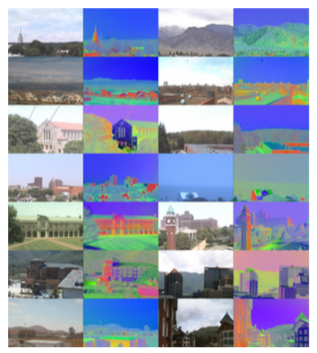
\includegraphics[scale=0.55]{amos-pca}
\centering
\caption{Image: a collection of pairs of an example image from a camera, and a false color image made from the first 3 components of the canonical day decomposition - the colors indicate sky (light blue), trees (light green), eastward facing wall (orange), westward facing wall (blue). From~\cite{many-outdoor-scenes}.}
\label{fig:amos}
\end{figure}

The authors of~\cite{many-outdoor-scenes} wanted to extend these findings to comparisons of cameras. In order to do this, they applied the same technique, but used average images for each camera as representations of the camera, and calculated the principal components of each camera. The SVD of these images showed that while the principal components were strongly dependent on the scene, the coefficient matrices of different cameras were similar. It was found that the variations were due to factors such as differences in dawn/dusk time between cameras and column permutations due to different types of variation in the scene (structural, temporal, etc). 

\section{Conclusion}
In this paper, we have described the process of PCA as a tool for understanding more about data than meets the eye, such as correlations in dimension as well as how these correlations can be used to reduce data dimensionality. We have also taken a deeper look into how PCA is used in the field of computer vision. PCA has become a popular tool for understanding basic coloration of images, as well as more interesting properties such as depth and structure of images. The use of PCA shows that the use of RGB values as dimensions can show far more than just coloration of images. 

\bibliographystyle{unsrt}
\bibliography{references}
\end{document}
